\section{Discussion and Future Work}

% Authors should discuss the results and how they can be interpreted from the perspective of previous studies and of the working hypotheses. The findings and their implications should be discussed in the broadest context possible. Future research directions may also be highlighted.


% \subsection{Model-Specific Limitations of GAN-Based Translation}
% \label{chapter:limitations}
Despite the remarkable performance achieved by the proposed framework, specific limitations remain. Since the translation relies solely on SAR data, which inherently contains speckle noise, the trained model struggles to generate realistic optical images when the SAR inputs lack distinct structural information. In such cases, the model appears unable to discern meaningful spatial patterns and instead interprets some parts of the scene as noise, resulting in noise-like optical outputs, as illustrated in Figure~\ref{fig:limitation_noise}.


\begin{figure}[h!]
    \centering
    \setlength{\tabcolsep}{2pt}
    \begin{tabular}{c *{3}{c}}
        % ------------------- Row 1 -------------------
        (i) & (ii) & (iii)\\
        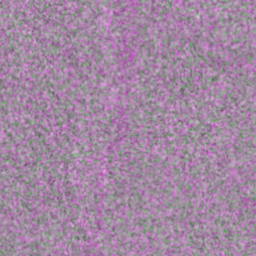
\includegraphics[width=0.2\textwidth, height=0.2\textheight, keepaspectratio]{../latex_source_code/img/limitation_noise/sample_000071_sar_pseudo.png} &
        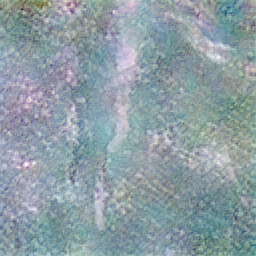
\includegraphics[width=0.2\textwidth, height=0.2\textheight, keepaspectratio]{../latex_source_code/img/limitation_noise/sample_000071_pred_rgb.png} &
        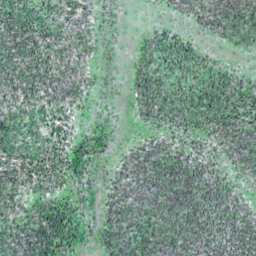
\includegraphics[width=0.2\textwidth, height=0.2\textheight, keepaspectratio]{../latex_source_code/img/limitation_noise/sample_000071_true_rgb.png} \\
        % ------------------- Row 2 -------------------
        
        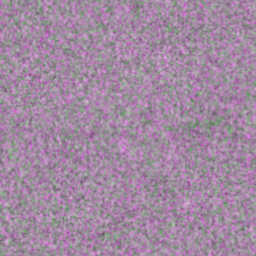
\includegraphics[width=0.2\textwidth, height=0.2\textheight, keepaspectratio]{../latex_source_code/img/limitation_noise/sample_000834_sar_pseudo.png} &
        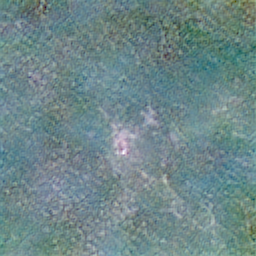
\includegraphics[width=0.2\textwidth, height=0.2\textheight, keepaspectratio]{../latex_source_code/img/limitation_noise/sample_000834_pred_rgb.png} &
        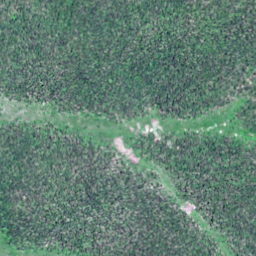
\includegraphics[width=0.2\textwidth, height=0.2\textheight, keepaspectratio]{../latex_source_code/img/limitation_noise/sample_000834_true_rgb.png} \\
    \end{tabular}

    \caption[Model limitation on structureless SAR inputs]{%
    Qualitative examples illustrating the limitation of the SAR-to-optical translation model when the SAR input lacks clear structural information. 
    Columns: 
    \textbf{(i)}~SAR input, 
    \textbf{(ii)}~model-generated optical image, and 
    \textbf{(iii)}~reference cloud-free Sentinel-2 image. 
    }
    \label{fig:limitation_noise}
\end{figure}

To address these generative artifacts, future research should consider alternative architectures such as Diffusion Models. Unlike GANs, which can suffer from training instability, diffusion models explicitly learn to reverse noise processes to synthesize data. Recent state-of-the-art performance on the SEN12-MS-CR dataset by methods like \textit{DiffCR}~\cite{DiffCR} suggests that diffusion-based approaches~\cite{c_diffusion_s2o, s2o_color_super_diff, SAR_DeCR, strgb_lat_diff} may offer superior fidelity and stability for SAR-to-optical translation. Additionally, performance could be enhanced by integrating attention mechanisms. Approaches such as the Spatial Attention GAN (SpA-GAN)~\cite{CR_RS_spati_atten_GAN} demonstrate that adaptively weighting features allows the network to prioritize relevant spatial details while suppressing noise or occlusions. Incorporating similar attention modules into SAR-to-optical architectures would likely improve feature consistency and spectral accuracy in complex scenes.


Beyond that, reducing noise in both image domains as much as possible before training and application could enhance the results as well. Since the imaging instruments are based on completely different technologies, different types of noise occur in principle. However, the different signal characteristics generate different noise through interactions with the Earth’s surface and the atmosphere: while SAR noise is mostly induced by backscattering effects, optical noise is rather caused by the atmosphere’s water content and other aerosols. The incompatibility of noise between both domains remains a challenge in AI-based SAR-to-optical translation.

The results demonstrate the potential of genAI-based methods to fill data gaps in a given image domain by data from another image domain. Since the methods are not restricted to SAR and optical images, they could also be applied for other purposes, such as the reconstruction of historic images, or translating between image data of different spectral characteristics, such as multi-spectral, hyperspectral, RGB or B/W.
% \textcolor{red}{TODO: add future work from Peter's suugestions!}



